\documentclass{article}\usepackage{hyperref}\usepackage{graphicx}\usepackage{amsmath}\usepackage{amsfonts}\newcommand{\deq}{\stackrel {\rm def}{=}} \newcommand{\eqline}[1]{\\\centerline{$#1$}\\}\newcommand{\tab}{\hphantom{6mm}}\newcommand{\well}[1]{\vspace{0.3cm}\hspace{-2cm}{\tt #1}} \begin{document}

\section*{Introduction}

\subsection*{Problem position}

Automated machine learning\footnote{The notions of ``\href{https://en.wikipedia.org/wiki/Automated\_machine\_learning}{automated-machine-learning}'', ``\href{https://en.wikipedia.org/wiki/Meta_learning_(computer_science)}{meta-learning}'', including ``\href{https://en.wikipedia.org/wiki/Meta-optimization}{meta-optimization}'' and ``\href{https://en.wikipedia.org/wiki/Hyperparameter_(machine_learning)}{hyperparameter}'' and the related ``\href{http://neupy.com/2016/12/17/hyperparameter\_optimization\_for\_neural\_networks.html}{hyperparameter optimization}'', have precise meaning in machine-learning, and we assume this is known to the reader.} is ``the process of automating the end-to-end process of machine learning'', because the complexity of adjusting the hyperparameters, including selecting a suitable method, becomes easily time-consuming when not intractable. To this end, the general idea is to consider a standard machine-learning algorithm and to add on ``top of it'' another algorithmic mechanism, e.g., another machine learning algorithm dedicated to automatic hyperparameter adjustment, with the caveat of generating other hyperparameters for the meta-learning algorithm and without formal guaranty that this accumulation of mechanisms is optimal.

The key setting is to adjust the model parameter by optimizing the criterion on a {\em learning} data set, and validate the hyperparameter choice by rerunning the optimization for different hyperparameter values on a different {\em validation} data set, while the final performance is evaluated on another {\em test} set. 
Hyperparameter tuning is mainly required to maximize predictive accuracy, i.e., not only optimize the learning on the present data set, but also generalize this learning to subsequent data. Another goal is to not only adjust one model parameter set, but also to adapt the model itself.

Here we propose to follow another track:  How is it possible to consider the automatic adjustment of hyperparameters not as a separate process but within the learning algorithm itself ? Let us call such parameters {\em meta-parameters} and let us attempt to formalize such an alternative track.

\subsection*{Related work}

As being an everyday concrete problem for the machine learning community, there is a huge literature on hyperparameter adjustment of optimization algorithms. A recent review of automatic selection methods for machine learning algorithms and hyperparameter values is available \cite{luo2016review}, while the state of the art regarding hyper-heuristics has been made by \cite{burke2013hyper}, an introducing overview about automatic hyperparameter optimization and model selection for supervised machine learning is available in this student work \cite{bermudez2014automatic}. Hyperparameter adjustment packages are available with every machine learning framework, searching through the joint space of hyperparameter settings such as, e.g., Hyperopt \cite{bergstra2013hyperopt} or, e.g., Auto-WEKA \cite{kotthoff2017auto}. They are mainly based on Bayesian optimization method (beyond grid-search or random-search), considering that the cost of one optimization is high, while searching in the hyper-parameter space given a small data set of previous knowledge regarding hyper-parameter performance can highly improve the final result. Such search is based on a surrogate model of the optimization algorithm, using, e.g., tree-structured Parzen estimator \cite{bergstra2011algorithms} or Gaussian process \cite{snoek2012practical} (see \cite{qin2017improving} for a discussion and an important improvement).

Beyond these vanilla methods, several non-trivial improvements have been proposed. Hyperparameters can be updated before model parameters have fully converged (e.g., \cite{pedregosa2016hyperparameter}) interpolating the final optimization criterion value. Train-test samples can be matched across candidate hyperparameter configurations, allowing early elimination of sub-optimal candidates to minimize the number of evaluations and avoiding full cross-validation, with hypothesis testing embedding in the search algorithm \cite{zheng2013lazy}. Cross-validation based protocols with simultaneous hyperparameter optimization is proposed by several authors, e.g., \cite{tsamardinos2015performance}. The key idea of such collaborative hyper-parameter tuning methods \cite{bardenet2013collaborative}, is to design interaction between several hyperparameter evaluation \cite{jamieson2016non}, yielding an unbounded armed bandits problem \cite{li2016efficient}. Among sophisticated hyperparameter adjustment methods exact gradients of cross-validation performance with respect to hyperparameters (chaining derivatives backwards through the training procedure) has been proposed \cite{maclaurin2015gradient}, while hyper-optimization that transfers information by constructing a common response surface for all data set has been developed \cite{yogatama2014efficient}. This tiny review is only illustrative and far from being exhaustive: the topic is really huge (consider, for instance, that this also raise problems of data privacy in the sense of not inferring private data from repeated optimization output \cite{kusner2015differentially}).

In deep link with this issue, authors also consider adaptively learning the model architecture itself \cite{cortes2016adanet}. Automatic model design can be specified as searching for an optimal sub-graph within a large computational graph \cite{pham2018efficient}, these authors using parameter sharing between alternatives to improve the performances. More generally multi-model estimation methods (e.g., \cite{vieville:inria-00000172}) introduce qualitative hyperparameters to adjust.

Finally, another track is to consider algorithms for which hyper-parameter tuning is requires little tuning (e.g., considering the ADAM approach of \cite{kingma2014adam}, where the first-order gradient-based optimization of stochastic objective functions is based on adaptive estimates of lower-order momenta, or improving vanilla or natural gradient methods by automatic adjustment of the local optimization \cite{marceau2016practical}). This includes changing the algorithm itself (e.g., replacing k-mean clustering algorithms, by hierarchical clustering methods).

\subsection*{Proposed contribution}

Let us explore here a rather disruptive track, with respect to these complex issues: What about ``hyperparameterless'' machine learning methods ? In order to draft such approach we are first going to make the distinction between several kind of hyperparameters and claim that the solution depends on such distinction. We then are going to point out that the lever is to introduce as much as possible a-priori information in the machine learning process, indeed, but not at the level decreed by a given method, whereas at the level of the learning design. We further are going to get inspired by the way the brain adjust its ``meta-parameters'' and propose to consider machine learning not only as parameter optimization with meta-learning on a validation set, but as more fexible multi-loop architecture. 

In order to address such issue, we focus on a precise hybrid learning task (mixing supervised and reinforcement learning), with the idea of considering not-so-big data set as discussed in \cite{Drumond2017From}.

\section*{Problem setting}

\subsection*{Notations}

To develop our idea we are going to consider a simple input-output transformation :
\eqline{{\bf o} = {\bf f}_{\bf w}({\bf i}),}
mapping an input ${\bf i} \in {\cal R}^I$ onto an output ${\bf o} \in {\cal M} \subset {\cal R}^O$, as a function of parameters (e.g., network weights or architecture size) ${\bf w} \in {\cal R}^W$, and a sequence of input ${\bf i}_n, t \in \{1, N\}$, coupled with a output loss function sequence $l_n(\cdot)$ with the goal to minimize the loss expectation: 
\eqline{{\bf w}^\bullet = \mbox{arg max}_{\bf w} \mathbb{E}[l({\bf f}_{\bf w}({\bf i}))]}
and would like, given a learning set, to minimize this expectation on subsequent input.

The computed values lives in a compact (thus bounded) subset ${\cal M} \subset {\cal R}^O$. The extrinsic dimension $O$ is expected to be large. Qualitative values simply corresponds to discrete components of ${\cal M}$.

\subsection*{Basic issues}

Such a setup corresponds to standard supervized learning, e.g., considering a classification task, the output including both the sample label and its internal feature representation. Labeled and unlabeled samples can be taken into account, the former corresponding to a zero loss function. Temporal sequence learning and reinforcement learning does not directly fit in this setup (except if considering temporal or policy sequences as a whole), but generalization to these paradigms is kept in mind by the authors and will be an interesting extension of this work.

As formalized, by the no free-lunch theorem for optimization \cite{wolpert1997no}, a general-purpose, universal optimization strategy is impossible. The only way one strategy can outperform another is if it is specialized to the structure of the specific problem under consideration. Futhermore, such problem lives in a huge dimensional space, with is known to impair such optimization task, especially as far as generalization is concerned (see, e.g., \cite{trunk1979problem} for an illustrative example or classical works such as \cite{vapnik2013nature}).

Let us see how to overcome this double curse, by suitable design choices.

\subsection*{Considering different classes of parameters}

The standard learning setup consists of a model, with model parameters to adjust on the data, thee design of the model being 

\begin{figure}[htb]
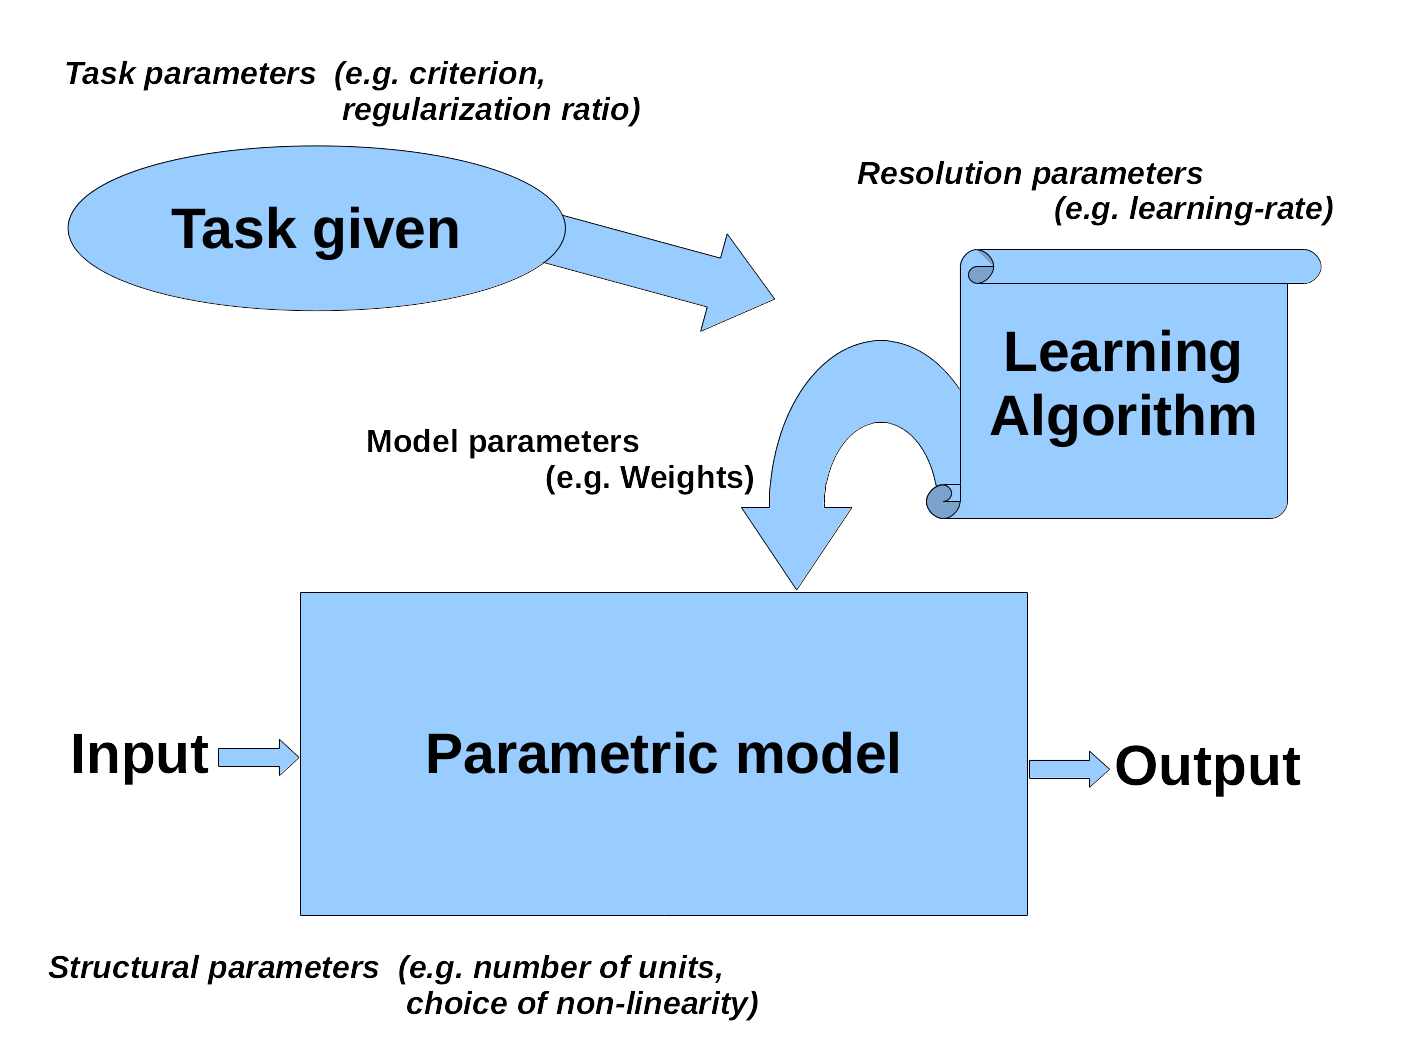
\includegraphics[width=0.9\textwidth]{img/hyperparameters}
\caption{Three kinds of hyperparameters, related to either the learning task, the proposed model, or the estimation algorithms. Automatizng the adjustment of these parameters highly depends on these three classes.}
\label{hyperparameters}
\end{figure}



%Considering, e.g., deep networks, meta-parameters include structural parameters (such as  the choice of the loss function and the parameters of the regularization part of such loss function, or the parameter initialization method. The effect of all these values can not be observed from one step to another, but considering a whole epoch (i.e., a training cycle on the training set). This the case of the batch-size and epoch-duration in our example. 

Our first design choice is to make a strong distinction between: \begin{itemize}

\item {\em Structural parameters}: These are the hyper-parameters related to the model design choice, usually fixed before the learning starts. For a deep networks, the number of layers, and within a layer the number of units (hidden units and output units), the unit connection size (e.g. convolution layer filter size) and/or form, the choice of the non-linearity (i.e., of the activation function) are such parameters. For a reservoir computing network, the parameters used to draw the fixed recurrent random weights (i.e., the choice of the weight distribution and its standard-deviation, yielding the reccurent matrix weigt spectral radius) are typical structural parameters.  \begin{itemize}

 \item Our claim is that, as in multi-model estimation methods, such hyperparameters can be considered as model p[a

\bibliographystyle{alpha}\bibliography{../bib/vthierry} \end{document}
